
\begin{figure}[ht]
 \centering
  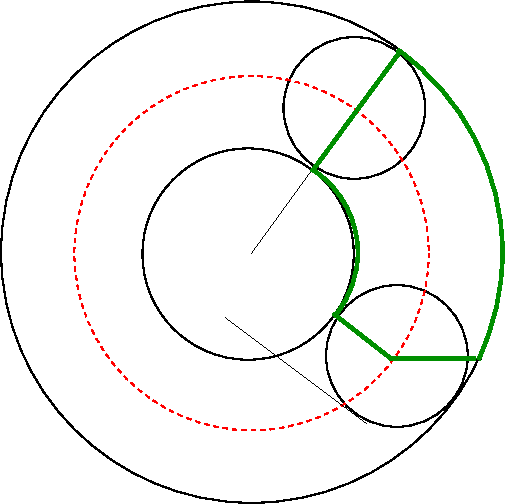
\includegraphics{Cplanimetre_1.pdf}
 \caption{Domaine $\Omega$}
 \label{fig:Cplanimetre_1}
\end{figure}

\begin{enumerate}
 \item L'ensemble des points que peut atteindre l'extrémité de la deuxième tige est la couronne entre les cercles de rayon $R-r$ et $R+r$. Dans cette couronne, chaque point $m$ peut être atteint de deux manières. Il suffit de tracer le cercle centré en $m$ et de rayon $r$. Il coupe le cercle de rayon $R$ (formé par les positions possibles de l'extrémité de la première tige) en deux points.
\item Il n'est pas facile de préciser le plus grand domaine $\Omega$ possible. On se contentera du domaine délimité par le bord vert sur la figure \ref{fig:Cplanimetre_1}.
\item On trouve sans problème particulier

\begin{multline*}
\left\lbrace 
\begin{aligned}
x &= R\cos \alpha +r \cos \beta \\
y &= R\sin \alpha +r \sin \beta  
\end{aligned} 
\right. 
\Rightarrow
\left\lbrace 
\begin{aligned}
dx &= -R\sin \alpha \,d\alpha -r \sin \beta \,d\beta\\
dy &= R\sin \alpha \,d\alpha + r \cos \beta \,d\beta\\ 
\end{aligned}
\right. \\
  \Rightarrow dx\wedge dy = Rr\sin(\beta-\alpha)\, d\alpha \wedge d\beta 
\end{multline*}

\item 
Le coefficient de $d\alpha$ dans $\omega$ est le produit scalaire
\begin{displaymath}
(\begin{pmatrix}
-R\sin \alpha\\
R\cos \alpha
  \end{pmatrix}
/
\begin{pmatrix}
-\sin \beta\\
\cos \beta
  \end{pmatrix} )
\end{displaymath}
Celui de $d\beta$ est clairement $1$ donc $\omega=d\beta +R\cos(\beta-\alpha)d\alpha$ et :
\[d\omega= R\sin(\beta-\alpha)d\alpha \wedge d\beta=dx\wedge dy\]
Par conséquent l'intégrale curviligne de $\omega$ le long du contour fermé est l'aire du domaine. Cette intégrale est aussi la distance parcourue par la roulette à cause de la définition même de la forme $\omega$.
\end{enumerate}
